\graphicspath{{../../S13_Expressions_litterales/Images/}}

\themeN
\chapter{Expressions littérales}
\label{S13}

\programme%
   {\item Notion d'inconnue.}
   {\item Utiliser le calcul littéral pour traduire une propriété générale, pour démontrer un résultat général, pour valider ou réfuter une conjecture, pour modéliser une situation.}

\vfill

\begin{debat}{Débat : petits contes mathématiques}
   Les vidéos des {\bf Petits contes mathématiques} ont été créés par {\it Universciences} : c'est une série pédagogique qui retrace l'histoire des maths à travers la découverte d'une notion, d'une formule, d'une conjecture ou d'une équation. Le récit est rythmé par des illustrations animées et la légèreté du ton dédramatise le sujet pour tous ceux qui ne seraient pas des \og matheux \fg.
   \tcblower
      \begin{pspicture}(0,0)(5,3)
         \rput{10}(1,1){\huge $x$}
         \rput{20}(3.5,2.25){\huge $y$}
         \rput{-10}(3,0.5){\huge $z$}
         \rput(0.5,2.5){\huge $+$}
         \rput(2,1.5){\huge $\times$}
         \rput(4.5,2){\huge $()$}
         \rput(5,0.75){\huge $-$}
         \rput(2,3){\huge $\div$}
         \rput{-20}(5,3){\huge $t$}
      \end{pspicture}
\end{debat}

\hfill {\gray Vidéo : \href{https://leblob.fr/fondamental/le-x}{\bf Le $x$}, site Internet {\it Le blob}, épisode de la série {\it Petits contes mathématiques}.}


%%% Approche %%%
\begin{Maquette}[Cours]{Theme={Activité d'approche},Couleur={SteelBlue}}

   \AAtitre{Des variables aux inconnues}

      {\it Objectifs : voir l'effet des variables dans un programme de calcul créé avec Scratch ; produire une expression littérale.}

      \begin{AActivite}

         On considère le programme de calcul ci-dessous dans lequel $x$, Etape 1, Etape 2 et Résultat sont quatre variables.
         \begin{center}
            \begin{Scratch}[Echelle=0.9]
               Place Drapeau ;
               Place Demander("Choisis un nombre");
               Place MettreVar("x",OvalCap("réponse"));
               Place DireT("Je multiplie le nombre par 6.","2");
               Place MettreVar("Etape 1",OpMul("6",OvalVar("x")));
               Place DireT("J'ajoute 10 au résultat.","2");
               Place MettreVar("Etape 2",OpAdd(OvalVar("Etape 1"),"10"));
               Place DireT("Je divise le résultat par 2.","2");
               Place MettreVar("Résultat",OpDiv(OvalVar("Etape 2"),"2"));
               Place Dire(OpRegrouper("J'obtiens finalement",OvalVar("Résultat")));
            \end{Scratch}
         \end{center}
         \begin{enumerate}
            \item Yasmina a fait fonctionner ce programme en choisissant le nombre 5.\par
            Vérifier que ce qui est dit à la fin est : \og J’obtiens finalement 20 \fg. Pour cela, remplir le diagramme suivant : \par
               \begin{pspicture}(-3,-0.1)(8,1.8)
                  \psframe(0,0.5)(1,1.5)
                  \rput(0.5,0){$x$}
                  \psline[arrowsize=2mm]{->}(1.1,1)(2.4,1)
                  \psframe(2.5,0.5)(3.5,1.5)
                  \rput(3,0){étape 1}
                  \psline[arrowsize=2mm]{->}(3.6,1)(4.9,1)
                  \psframe(5,0.5)(6,1.5)
                  \rput(5.5,0){étape 2}
                  \psline[arrowsize=2mm]{->}(6.1,1)(7.4,1)
                  \psframe(7.5,0.5)(8.5,1.5)
                  \rput(8,0){résultat}
               \end{pspicture}         
            \item Que dit le programme si Maissa le fait fonctionner en choisissant au départ le nombre 7 ? \par
               \begin{pspicture}(-3,-0.1)(8,1.8)
                  \psframe(0,0.5)(1,1.5)
                  \rput(0.5,0){$x$}
                  \psline[arrowsize=2mm]{->}(1.1,1)(2.4,1)
                  \psframe(2.5,0.5)(3.5,1.5)
                  \rput(3,0){étape 1}
                  \psline[arrowsize=2mm]{->}(3.6,1)(4.9,1)
                  \psframe(5,0.5)(6,1.5)
                  \rput(5.5,0){étape 2}
                  \psline[arrowsize=2mm]{->}(6.1,1)(7.4,1)
                  \psframe(7.5,0.5)(8.5,1.5)
                  \rput(8,0){résultat}
               \end{pspicture}         
            \item Firdaws fait fonctionner le programme, et ce qui est dit à la fin est : \og J’obtiens finalement 8 \fg. Quel nombre a-t-elle choisi au départ ? \par
               \begin{pspicture}(-3,-0.1)(8,1.2)
                  \psframe(0,0.5)(1,1.5)
                  \rput(0.5,0){$x$}
                  \psline[arrowsize=2mm]{<-}(1.1,1)(2.4,1)
                  \psframe(2.5,0.5)(3.5,1.5)
                  \rput(3,0){étape 1}
                  \psline[arrowsize=2mm]{<-}(3.6,1)(4.9,1)
                  \psframe(5,0.5)(6,1.5)
                  \rput(5.5,0){étape 2}
                  \psline[arrowsize=2mm]{<-}(6.1,1)(7.4,1)
                  \psframe(7.5,0.5)(8.5,1.5)
                  \rput(8,0){résultat}
               \end{pspicture} 
            \item Si l’on appelle $x$ le nombre choisi au départ, écrire en fonction de $x$ l’expression obtenue à la fin du programme. \par
               \begin{pspicture}(-3,0.1)(8,1.8)
                  \psframe(0,0.5)(1,1.5)
                  \rput(0.5,1){$x$}
                  \psline[arrowsize=2mm]{->}(1.1,1)(2.4,1)
                  \psframe(2.5,0.5)(4,1.5)
                  \rput(3.25,0){étape 1}
                  \psline[arrowsize=2mm]{->}(4.1,1)(5.4,1)
                  \psframe(5.5,0.5)(7.5,1.5)
                  \rput(6.5,0){étape 2}
                  \psline[arrowsize=2mm]{->}(7.6,1)(8.9,1)
                  \psframe(9,0.5)(12,1.5)
                  \rput(10.5,0){résultat}
               \end{pspicture} 
         \end{enumerate}

      \end{AActivite}

      \vfill\hfill{\it\footnotesize Source : cette activité est une adaptation du DNB 2017 de Pondichery.}

\end{Maquette}


%%%Trace écrite %%%
\begin{Maquette}[Cours]{Theme={Trace écrite},Couleur={0.4[SteelBlue,Black]}}

   %%%1
   \section{Expressions littérales}
   
      \begin{definition*}{}
         Une {\bf expression littérale} est une succession d'opérations où apparaissent des lettres représentant des nombres. \par
         On parle aussi d'{\bf expression algébrique}.
      \end{definition*}
      
      \begin{exemple*}{}
         $4\times x+3$ \; ; \; $2\times a-89$ \; ; \; $y-3\times z+t-4$.
      \end{exemple*}
   
   
   %%%2
   \section{Produire une expression littérale}
   
      On utilise notamment des expressions littérales pour produire des  formules générales, qui pourront être utilisées quelle que soit la valeur des variables.
      
      \begin{exemple*}{}
         \begin{itemize}
            \item Matéo a quatre ans de plus que Noé. \par
               En appelant \og $x$ \fg{} l'âge de Noé, l'âge de Matéo peut s'écrire \og $x+4$ \fg.
            \item Un rectangle a pour largeur $\ell$ et pour longueur $L$. \par
               Son périmètre peut s'exprimer ainsi : $\mathcal{P} =2\times(\ell+L)$. \par
               Son aire peut s'exprimer ainsi : $\mathcal{A} =\ell\times L$. \par
         \end{itemize}
      \end{exemple*}
      
      Remarque : la circonférence d'un disque s'écrit $2\pi R$ où :
         \begin{itemize}
            \item $\pi$ est une lettre grecque qui désigne le nombre 3,14\dots, qui est fixe ;
            \item $R$ est une lettre qui désigne le rayon du disque, ce nombre est variable et dépend du disque.
         \end{itemize}
   
   
   %%%%3
   \section{Simplifier d'une expression littérale}
   
   Pour simplifier une expression littérale, on peut supprimer le signe \og $\times$ \fg{} devant une lettre, une parenthèse ou entre deux lettres. 
   
   \begin{propriete*}{}
      \begin{itemize}
         \item On utilise la notation $2a$ pour $a+a$ ou $a\times2$ ou encore $2\times a$. On dit \og deux a \fg.
         \item On utilise la notation $ab$ pour $a\times b$. On dit \og ab \fg.
         \item On utilise la notation $a^2$ pour $a\times a$. On dit \og a au carré \fg.
         \item On utilise la notation $a^3$ pour $a\times a\times a$. On dit \og a au cube \fg.
      \end{itemize}
   \end{propriete*}

   
   On écrit une expression comportant un nombre et une \og lettre \fg{} avec le nombre précédé de la \og lettre \fg.
   
   \begin{exemple*}{}
      Simplifier les expressions : \par
      $A =5\times y-2\times x =5y-2x$ \par
      $B =x\times x \times x + 7\times y\times y =x^3+7y^2$. \par
      $C =x\times3 =3x$, est préférable à $C=x3$. \par
         Par commutativité de la multiplication, $x\times3 =3\times x =3x$.
   \end{exemple*}

\end{Maquette}


%%% Exercices %%%
\begin{Maquette}[Fiche,CorrigeFin,Colonnes=2]{}

   \begin{multicols}{2}

      \begin{exercice} %1
         Si $x$ représente un nombre, comment peut-on écrire les expressions suivantes :
         \begin{enumerate}
            \item Le double de $x$.
            \item Le tiers de $x$.
            \item La somme de $x$ et de 13.
            \item La différence de $x$ et de 7.
            \item Le triple de la somme de 2 et de $x$.
            \item Le tiers de la différence de 16 et $x$.
         \end{enumerate}
      \end{exercice}
         
      \begin{Solution}
         \begin{enumerate}
            \item $2\times x =\cor{2x}$ \smallskip
            \item $\dfrac13\times x =\cor{\dfrac13x =\dfrac{x}{3}}$ \smallskip
            \item $\cor{x+13}$
            \item $\cor{x-7}$
            \item $3\times(2+x) =\cor{3(2+x)}$ \smallskip
            \item $\dfrac13\times(16-x) =\cor{\dfrac13(16-x) =\dfrac{16-x}{3}}$
         \end{enumerate}
      \end{Solution}
      

      \begin{exercice} %2
         Si on note $z$ l'âge en années de Zahra aujourd’hui, comment peut-on noter :
         \begin{enumerate}
            \item L'âge qu'elle aura dans deux ans ?
            \item Le triple de l'âge qu'elle avait il y a quatre ans ?
            \item La moitié de l'âge qu'elle aura dans cinq ans ?
            \item Son année de naissance si on est en 2024 ?
         \end{enumerate}
      \end{exercice}
      
      \begin{Solution}
         \begin{enumerate}
            \item $\cor{z+2}$
            \item $\cor{3(z-4)}$
            \item $\cor{\dfrac12(z+5) =\dfrac{z+5}{2}}$ \smallskip
            \item $\cor{2024-z}$
         \end{enumerate}
      \end{Solution}
      
      
      \begin{exercice}[SLF] %3
         Recopier les expressions suivantes en supprimant les signes $\times$ s'ils ne sont pas nécessaires.
         \begin{itemize}
            \item $A =9\times n =\pointilles$ \medskip
            \item $B =x\times3 =\pointilles$ \medskip
            \item $C =12\times(a-3) =\pointilles$ \medskip
            \item $D =2\times a(2\times8) =\pointilles$ \medskip
            \item $E =n\times x =\pointilles$ \medskip
            \item $F =2\times\pi\times R =\pointilles$ \medskip
         \end{itemize}
      \end{exercice}
      
      \begin{Solution}
         \begin{itemize}
            \item $A =9\times n =\cor{9n}$
            \item $B =x\times3 =\cor{3x}$
            \item $C =12\times(a-3) =\cor{12(a-3)}$
            \item $D =2\times a(2\times8) =2\times16a =\cor{32a}$
            \item $E =n\times x =\cor{nx}$
            \item $F =2\times\pi\times R =\cor{2\pi R}$
         \end{itemize}
      \end{Solution}

      
      \begin{exercice}[SLF] %4
         Simplifier les expressions suivantes :
         \begin{itemize}
            \item $A =a\times a =\pointilles$ \medskip
            \item $B =b\times b\times b =\pointilles$ \medskip
            \item $C =c\times c\times3 =\pointilles$ \medskip
            \item $D =9+d\times d\times d =\pointilles$ \medskip
            \item $E =a\times a\times b\times3 =\pointilles$ \medskip
            \item $F =x\times x\times x-2\times y\times y =\pointilles$ \medskip
            \item $G =(a+b)\times(a+b) =\pointilles$ \medskip
            \item $H =(x+y)(x+y)(x+y) =\pointilles$ \medskip
         \end{itemize}
      \end{exercice}
      
      \begin{Solution}
         \begin{itemize}
            \item $A =a\times a =\cor{a^2}$
            \item $B =b\times b\times b =\cor{b^3}$
            \item $C =c\times c\times3 =\cor{3c^2}$
            \item $D =9+d\times d\times d =\cor{9+d^3}$
            \item $E =a\times a\times b\times3 =\cor{3a^2b}$
            \item $F =x\times x\times x-2\times y\times y =\cor{x^3-2y^2}$
            \item $G =(a+b)\times(a+b) =\cor{(a+b)^2}$
            \item $H =(x+y)(x+y)(x+y) =\cor{(x+y)^3}$ \medskip
         \end{itemize}
      \end{Solution}
      
      
      \begin{exercice}[SLF] %5
         Dire si chaque affirmation est vraie ou fausse. \par \medskip
         \QCM[VF,Stretch=1.8,Largeur=1cm,NomV=vrai,NomF=Faux]{%
            $x\times x = 2x$&2,%
            $x+x = 2x$&1,%
            $x\times x =x^{2}$&1,%
            $x+x =x^{2}$&2,%
            $x+2 =2x$&2,%
            $x+2=x^{2}$&2,}
      \end{exercice}
      
      \begin{Solution}
         \QCM[VF,Stretch=1.8,Largeur=1cm,NomV=vrai,NomF=Faux,Solution]{%
            $x\times x = 2x$&2,%
            $x+x = 2x$&1,%
            $x\times x =x^{2}$&1,%
            $x+x =x^{2}$&2,%
            $x+2 =2x$&2,%
            $x+2=x^{2}$&2,}
      \end{Solution}
      
      
      \begin{exercice} %6
         Voici un programme :
         \begin{center}
            \ProgCalcul[Enonce,Largeur=4.5cm]{
               Choisis un nombre,
               Retire-lui 5,
               Multiplie le résultat par 3}
         \end{center}
         \begin{enumerate}
            \item Faire fonctionner le programme avec trois nombres de son choix supérieurs ou égaux à 5.
            \item Quel nombre faut-il choisir pour obtenir 6 ?
            \item Soit $x$ le nombre de départ, donner l'expression finale en fonction de $x$.
         \end{enumerate}
      \end{exercice}
      
      \begin{Solution}
         \begin{enumerate}
            \item \ProgCalcul{10,-5 *3}. \par
               Avec 10, on obtient \cor{15} \dots
            \item \ProgCalcul[Direct=false]{7,-5 *3}. \par
               On obtient 6 avec \cor{7}.
            \item \ProgCalcul[SansCalcul]{x,-5 *3,x-5 3(x-5)}. \par
               Ave$x$ on obtient \cor{$3(x-5)$}.
         \end{enumerate}
      \end{Solution}

      
      \begin{exercice}[Dur] %7
         Résoudre les défis suivants.
         \begin{enumerate}
            \item
               \begin{enumerate}
                  \item Choisir deux nombres consécutifs, calculer leur somme et comparer avec les résultats de la classe.
                  \item Quelle conjecture peut-on émettre ?
               \end{enumerate}
            \item On choisit un entier $n$.
               \begin{enumerate}
                  \item Comment s'écrit le nombre suivant $n$ ?
                  \item Donner l'expression de la somme de deux nombres consécutifs en fonction de $n$.
                  \item Démontrer la conjecture.
               \end{enumerate}
            \item Montrer que la somme de trois nombres consécutifs est multiple de 3.
         \end{enumerate}
      \end{exercice}
      
      \begin{Solution}
         \begin{enumerate}
            \item
               \begin{enumerate}
                  \item par exemple, \cor{$16+17 =33$}.
                  \item On peut conjecturer que  \cor{la somme de deux nombres consécutifs est un nombre impair}.
               \end{enumerate}
            \setcounter{enumi}{1}
            \item
               \begin{enumerate}
                  \item Le nombre suivant $n$ s'écrit \cor{$n+1$}.
                  \item $(n)+(n+1) =n+n+1 =\cor{2n+1}$.
                  \item $2n+1$ est un nombre pair ($2n$) auquel on ajoute 1, c'est donc un nombre impair. \\
                     \cor{La conjecture est vraie}.
               \end{enumerate}
            \setcounter{enumi}{2}
            \item Soit $n$ un nombre quelconque, le suivant s'écrit $n+1$ et celui d'après $n+2$. \\
               La somme de trois nombres consécutifs s'écrit alors : \\
               $(n)+(n+1)+(n+2) =n+n+1+n+2 =3n+3$. \\
               $3n+3$ est la somme de deux nombres multiples de 3, \cor{c'est donc un multiple de 3}.
         \end{enumerate}
      \end{Solution}

   \end{multicols}

\end{Maquette}


%%% Récré %%%
\begin{Maquette}[Cours]{Theme={Activité récréative},Couleur={IndianRed}}
    
   \ARtitre{Défis !!!}
   
      \parbox{2cm}{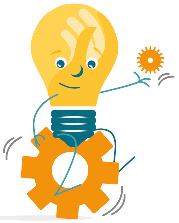
\includegraphics[width=2cm]{defi} \par \medskip
      \ARpartie{Défi 1}}
      \qquad
      \parbox{14cm}{
         Nihad et Adam ont choisi un nombre (entier positif). \par
         Nihad le multiplie par 5 et ajoute 35. \par
         Adam le multiplie par 2 et ajoute 146. \par
         Ils trouvent le même nombre à la fin. \par
         Quel nombre ont-ils choisi ?}
      
      \vfill
      
      \parbox{2cm}{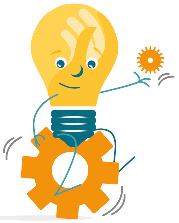
\includegraphics[width=2cm]{defi} \par \medskip
      \ARpartie{Défi 2}}
      \qquad
      \parbox{14cm}{
         Avec des petits carrés tous identiques, on construit un pattern selon le modèle évolutif ci-dessous : \par
         {\psset{unit=0.8}
         \begin{pspicture}(-3.5,-4.5)(4,3.75)
            \croix
            \rput(0.5,-2){Rang 1}
         \end{pspicture}
         \begin{pspicture}(-5,-4.5)(5,3.75)
            \croix
            \rput(2,0){\carre}
            \rput(0,2){\carre}
            \rput(-2,0){\carre}
            \rput(0,-2){\carre}
            \rput(0.5,-3){Rang 2}
         \end{pspicture}
         
         \begin{pspicture}(-8,-4.5)(4,1)
            \croix
            \rput(2,0){\carre}
            \rput(3,0){\carre}
            \rput(0,2){\carre}
            \rput(0,3){\carre}
            \rput(-2,0){\carre}
            \rput(-3,0){\carre}
            \rput(0,-2){\carre}
            \rput(0,-3){\carre}
            \rput(0.5,-4){Rang 3}
         \end{pspicture}}
         \begin{enumerate}
            \item Dessiner l’élément du rang suivant et expliquer la règle.
            \item Déterminer le nombre de petits carrés des éléments du rang 5, du rang 10, du rang 17.
            \item Déterminer le nombre de petits carrés de l’élément du rang 100 et donner un moyen de calculer rapidement le nombre de petits carrés d’un élément à n’importe quel rang.
            \item Existe-t-il un élément qui contient 532 petits carrés ? Un élément qui contient 813 petits carrés ?
         \end{enumerate}}
         
   \vfill\hfill {\it\footnotesize Source : \og La résolution de problèmes mathématiques au collège \fg, MENJS, 2021}

\end{Maquette}